\chapter{Конструкторский раздел}
\section{Общая схема метода}
Задача распознавания эмоций по звучащей речи сводится к соотношению исходных данные на входе (аудиозаписи звучащей речи) к определенному классу на выходе (виду эмоции). На рисунке \ref{fig:idef1} представлена IDEF0-диаграмма первого уровня решаемой задачи.
\begin{figure}[H]
	\centering
	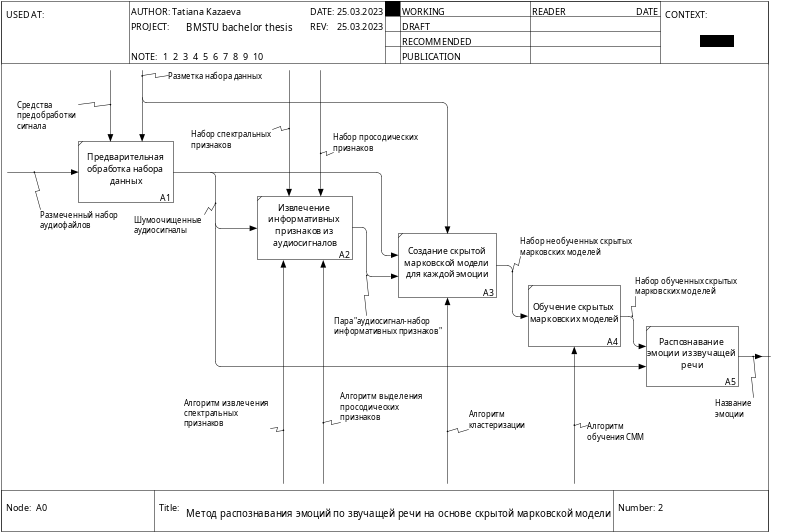
\includegraphics[width=\linewidth]{assets/02_A0}
	\caption{IDEF0-диаграмма первого уровня}
	\label{fig:idef1}
\end{figure}
Прежде всего набор данных должен быть предварительно обработан (блок А1).  Предварительная обработка включает в себя разделение набора данных на тренировочную (70-80\% набора) и тестовую (20-30\% набора) выборки.
Следующий этап решения задачи (блок А2) -- это извлечение информативных признаков из речевого сигнала.  Далее необходимо сократить размерность вектора информативных признаков. Для этого производится кластеризация векторов признаков сигналов (блок А3).  Этап создания и обучения скрытой марковской модели для каждой эмоции (блок А4) включает в себя определение количества состояний модели, а также вероятностей перехода между состояниями и вероятностей наблюдения признаков в каждом состоянии. В качестве состояний модели будут использованы порядковые номера выделенных кластеров. Обученную марковскую модель можно использовать для распознавания эмоций в звучащей речи (блок А5).
\section{Проектирование ключевых модулей системы}
%\subsection{Предварительная обработка данных}
%\subsection{Формирование обучающей выборки}
\subsection{Формирование вектора информативных признаков}
Самым надежным решением при распознавании эмоций в речи принято считать использование мел-кепстральных коэффициентов в качестве информативных признаков \cite{review}. В данной работе решено использовать первые 13 мел-кепстральных коэффициентов.

Формирование вектора информативных признаков, состоящего из 13-ти первых мел-кепстральных коэффициентов представлено на рисунке \ref{fig:mfcc-vector}.
\begin{figure}[H]
	\centering
	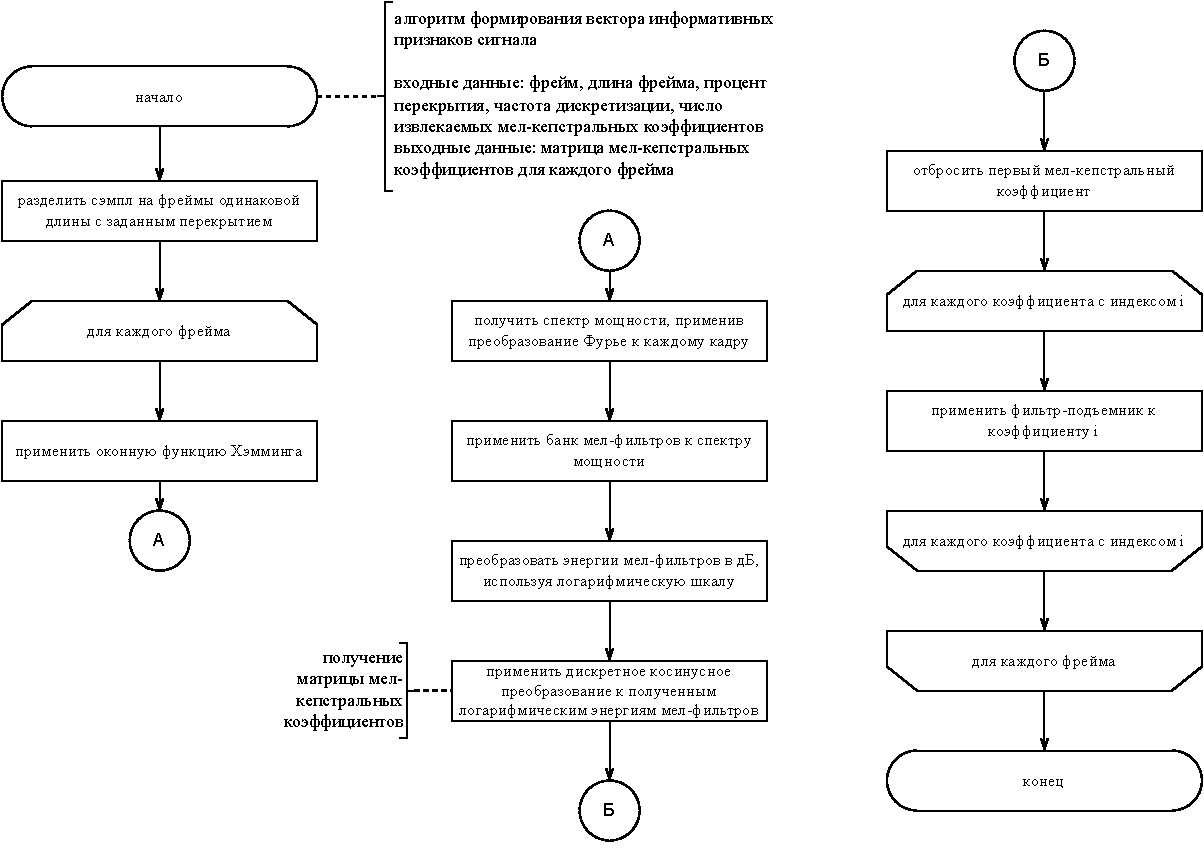
\includegraphics[width=\linewidth]{assets/mfccs-flowchart}
	\caption{Алгоритм формирования вектора информативных признаков}
	\label{fig:mfcc-vector}
\end{figure}

Фильтр-подъемник (lifter) применяется для усиления высокочастотных компонентов сигнала, которые могут быть утрачены в процессе преобразования сигнала в мел-кепстральные коэффициенты. Применение фильтра-подъемника происходит согласно \ref{eq:lifter}
\begin{equation}\label{eq:lifter}
	1 + \cfrac{\mathrm{lifter}}{2} \cdot \cfrac{\sin\left(\cfrac{\pi i}{\mathrm{lifter}}\right)}{1},
\end{equation}
где $i$ - индекс коэффициента MFCC, а $\mathrm{lifter}$ - значение параметра фильтра-подъемника.
\subsection{Кластеризация}
% В качестве алгоритма кластеризации был выбран k-means (\textit{англ. k-средних}).

Алгоритм k-means -- это неиерархичный метод неконтролируемого обучения. Он позволяет разделить произвольный набор данных на заданное число кластеров так, что объекты внутри одного кластера были достаточно
близки друг к другу, а объекты разных не пересекались. Цель этого алгоритма — объединить в группы сходные данные по некоторым заданным критериям. Чаще всего при кластеризации используются меры расстояния. В данной работе в качестве меры расстояния будет реализовано Евклидово (квадратичное) расстояние согласно \ref{eq:kdist}:
\begin{equation}\label{eq:kdist}
	\mathrm{dist}(p,\;q) = \sqrt{(p - q)^2},
\end{equation}
где $p, q$ -- точки вектора входных данных. Точка вектора входных данных имеет 13 измерений, поскольку точкой в данном случае являются значения мел-кепстральных коэффициентов, наблюдаемых на каждом фрейме каждого сэмпла.

Результатом работы алгоритма кластеризации является массив 13-ти мерных точек, являющихся центроидами каждого кластера. После получения центроидов необходимо определить ближайший центроид для каждого набора мел-кепстральных коэффициентов, полученного в модуле выделения информативных признаков. В результате работы всего модуля устанавливается соответствие <<кластер-фрейм>>, необходимое для дальнейшего обучения скрытой марковской модели.

Схема алгоритма кластеризации представлена на рисунке \ref{fig:kmeans}.
\begin{figure}[H]
	\centering
	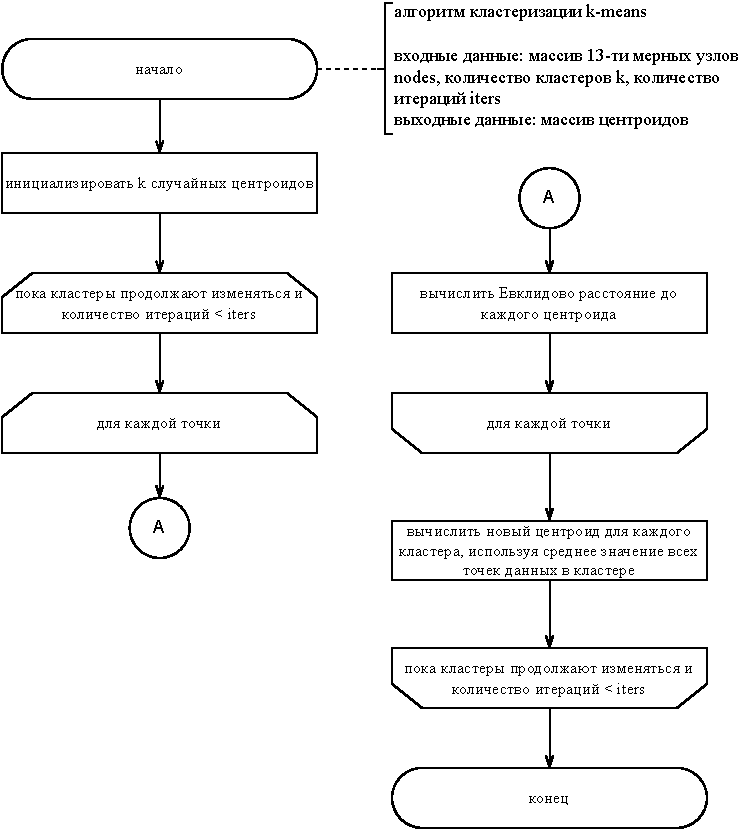
\includegraphics[width=0.7\linewidth]{assets/kmeans-flowchart}
	\caption{Алгоритм кластеризации k-means}
	\label{fig:kmeans}
\end{figure}

\subsection{Создание и обучение скрытых марковских моделей}
Обучение скртыой марковской модели -- это определение параметров $\lambda = \{A, B, \pi\}$ с учетом количества последовательностей наблюдений $\{O = O_1, \dots, O_n\}$. Для обучения скрытой  марковской модели используется алгоритм Баума --- Велша. Стоит отметить, что он применим только в том случае, если предварительно определено количество состояний и наблюдений.
%Алгоритм Баума-Велша состоит из трех этапов, для формализации которых следует ввести ряд обозначений.
Пусть $\gamma$ -- условная вероятность нахождения в определенном состоянии $q_i$ в с учетом последовательности наблюдений (\ref{hmm-gamma}):
\begin{equation}\label{hmm-gamma}
	\gamma_i = P(s_t = q_i\,|\,O,\,\lambda) = \cfrac{P(s_t = q_i,\,O\,|\,\lambda)}{P(O)}.
\end{equation}
Далее следует ввести переменную $\alpha$, обозначающую вероятность частичной последовательности наблюдений до момента времени $t$, находящаяся в состоянии $q_i$ в момент времени $t$, согласно \ref{hmm-alpha}:
\begin{equation}\label{hmm-alpha}
	\alpha_i = P(O_1, O_2, \dots, O_t,\, S_t = q_i\,|\,\lambda),
\end{equation}
и переменную $\beta$, вероятность частичной последовательности наблюдений от $t + 1$ до $T$, при нахождении в состоянии $q_i$ в момент времени $t$ (\ref{hmm-beta}): 
\begin{equation}\label{hmm-beta}
	\beta_i = P(O_{t+1}, O_{t+2}, \dots, O_T,\, S_t = q_i\,|\,\lambda),
\end{equation}
С учетом этих обозначений следует ввести переменную $\xi$, обозначающую вероятность перехода из состояния $i$ в момент времени $t$ в состояние $j$ в момент времени $t + 1$ с учетом последовательности наблюдений $O$ согласно \ref{hmm-xi}:
\begin{equation}\label{hmm-xi}
	\xi_t(i,\,j) = \frac{\alpha_t(i)a_{i,\,j}b_j(O_{t+1})\beta_{t+1}(j)}{P(O)}.
\end{equation}
С учетом переменных $\alpha$ и $\beta$ (\ref{hmm-alpha} и \ref{hmm-beta}) задать $\xi$ удобнее согласно \ref{hmm-xi-alpha-beta}:
\begin{equation}\label{hmm-xi-alpha-beta}
	\xi_t(i,\,j) = \alpha_t(i)a_{i,\,j}b_j(O_{t+1}\beta_{t+1}(j) \bigg/ \sum_{i}\sum_{j}\alpha_t(i)a_{i,\,j}b_j(O_{t+1}\beta_{t+1}(j)
\end{equation}
С учетом введенных обозначений, Баума---Велша можно разделить на 5 этапов.
\begin{enumerate}
	\item Выполнение прямого прохода, в результате которого вычисляются вероятности наблюдаемых последовательностей до каждого момента времени и вероятности переходов из одного скрытого состояния в другое.
	\item Выполнение обратного хода, в результате которого вычисляются апостериорные вероятности скрытых состояний в каждый момент времени.
	\item оценка априорных вероятностей -- количество случаев нахождения в состоянии $i$ в момент времени $t$ согласно \ref{eq:bw3}:
	\begin{equation}\label{eq:bw3}
		\pi_i = \gamma_1(i).
	\end{equation}
	\item  Оценка вероятностей переходов -- количество переходов из состояния  $i$ в состояние $j$ по отношению к количеству случаев нахождения в состоянии $i$ согласно \ref{eq:bw4}:
	\begin{equation}\label{eq:bw4}
		a_{i, j} = \cfrac{\displaystyle\sum_{t=1}^T \gamma_j(t) 1(v(t)=k)}{\sum_{t=1}^T \gamma_j(t)}.
	\end{equation}
	\item Оценка вероятностей наблюдений -- количество случаев нахождения в состоянии $j$ при количестве наблюдений $k$ по отношению к количеству случаев нахождения в состоянии $j$ согласно \ref{eq:bw5}:
	\begin{equation}\label{eq:bw5}
		b_{j,\,k} = \cfrac{\displaystyle\sum_{t=1}^T \gamma_j(t) 1(v(t)=k)}{\sum_{t=1}^T \gamma_j(t) }
	\end{equation}
\end{enumerate}
Алгоритм обучения скрытых марковских моделей представлен на рисунке \ref{fig:hmm-train}.
\begin{figure}[H]
	\centering
	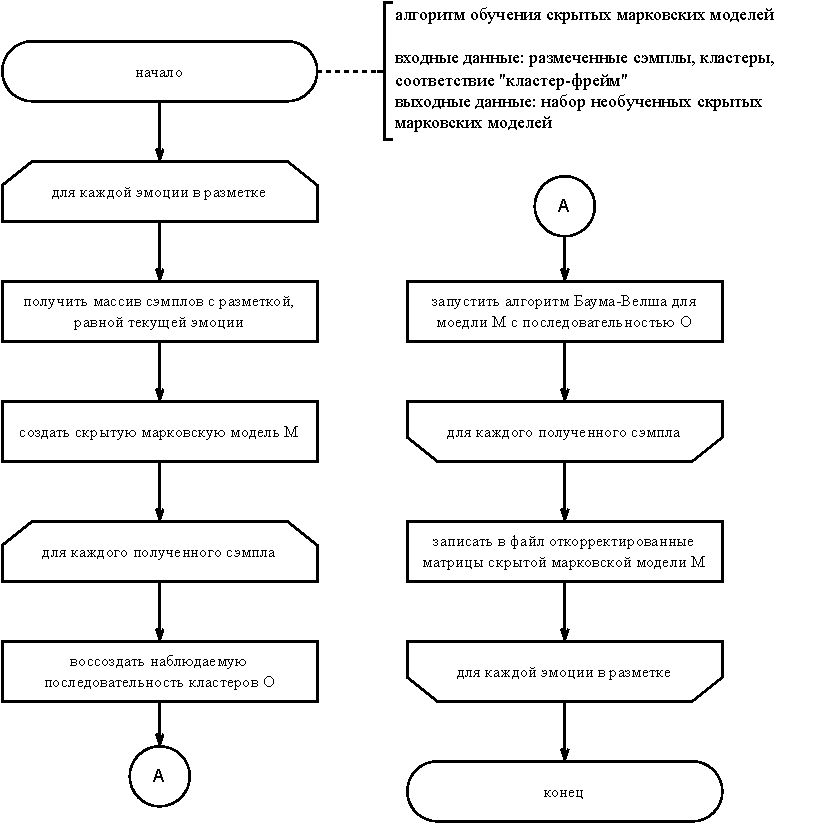
\includegraphics[width=0.8\linewidth]{assets/hmm-train}
	\caption{Обучение скрытых марковских моделей}
	\label{fig:hmm-train}
\end{figure}

\subsection{Определение эмоции из аудиосигнала}
Для того, чтобы выделить эмоцию из семпла, необходимо определить вероятности наблюдения последовательности кластеров семпла для каждой марковской модели. В алгоритме прямого прохода вычисляются не только вероятности $\alpha$, но также и вероятность наблюдать данную последовательность при условии заданной модели. Алгоритм представлен на листинге \ref{alg:forward}.
%
\begin{algorithm}[H]
	\KwData{Скрытая марковская модель $\lambda$; Последовательность наблюдений $O$; количество состояний $N$;  Количество наблюдений $T$}
	$i \leftarrow 0;\;$\For{ i < $T$}
	{
		$\alpha_1(i) = \pi_ib_i(O_1)$; // инициализация
	}
	
	$t \leftarrow 1;\;$\For{ t < $T$}
	{
		$j \leftarrow 0;\;$\For{ j < $N$}
		{
			$\alpha_t(j) = \displaystyle\sum_i\alpha_{t - 1}(i)a_{i,\,j}b_j(O_t)$ // индукция
		}
	}
	$P(O) = \displaystyle\sum_i\alpha_T(i)$
	\caption{Алгоритм прямого хода}
	\label{alg:forward}
\end{algorithm}
Алгоритм прямого прохода состоит из трех основных частей: инициализация, индукция и завершение. На этапе инициализации определяются переменные $\alpha$ для всех состояний в начальный момент времени. На этапе индукции вычисляются значения $\alpha_{t + 1}(i)$ по значениям $\alpha_t(i)$. На этапе завершения вычисляется значение $P(O\,|\,\lambda)$ путем суммирования всех значений $\alpha_T$.

Распознавание происходит следующим образом: для каждого семпла выделяется последовательность наблюдений, состоящая из номеров кластеров, присвоенных каждому фрейму семпла на этапе кластеризации. Для каждой обученной модели запускается алгоритм прямого прохода, из которого определяются вероятности наблюдения данной последовательности кластеров с учетом модели. Полученные вероятности сравниваются. Та модель, для которой вероятность наблюдения максимальная, считается подходящей. Алгоритм распознавания представлен на риснуке \ref{fig:hmm-test}.

\begin{figure}[H]
	\centering
	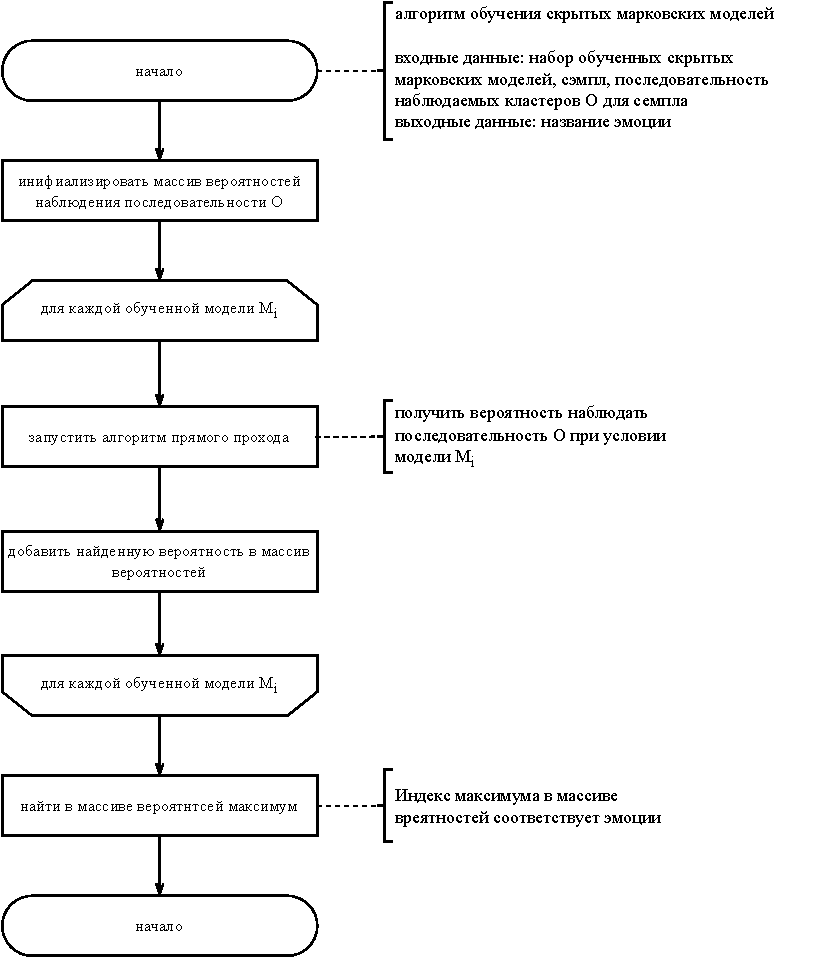
\includegraphics[width=0.7\linewidth]{assets/hmm-test}
	\caption{Выделение эмоции из аудиосигнала}
	\label{fig:hmm-test}
\end{figure}

\section{Описание используемого набора данных}
\subsection{Разметка и структура набора}
Для обучения классификатора было решено использовать набор данных DUSHA \cite{dusha}, содержащий записи эмоциональной речи. Набор разделен на два домена -- аудиоматериалы, собранные с помощью краудсорсинга (\textit{англ. <<Croud>>}) и выдержки из русскоязычных подкастов (\textit{англ. <<Podcast>>}). 

При разметке эмоциональных наборов данных существует сложность в неоднозначности интерпретации эмоции аннотаторами. В наборе данных DUSHA эта проблема решается привлечением к оцениванию двух независимых экспертных групп. В наборе присутствуют только те записи, для которых оценка обоих групп была консистентна. В разметке присутствуют следующие классы эмоций: 
\begin{itemize}
	\item \textbf{нейтраль};
	\item \textbf{позитив}: текст требовалось произносить с улыбкой или смехом, стараться делать выраженные ударения на позитивно окрашенных словах;
	\item \textbf{грусть}: произносить текст требовалось приглушенным голосом, меланхолично;
	\item \textbf{злость или раздражение}: текст требовалось произнести с криком или сквозь зубы, и, аналогично позитиву, стараться делать выраженные ударения на негативно окрашенных словах.
\end{itemize}

В домене <<Crowd>> тексты были искусственно сгенерированы на основе записей общения с голосовым ассистентом. Затем они были озвучены двумя способами: эмоционально, с той эмоцией, которую показал на этой записи классификатор BERT \cite{bert} и безэмоционально. Домен <<Podcast>> содержит уже не имитацию эмоции, а естественную речь. Все аудиозаписи были сделаны на профессиональные микрофоны, качество аудио было унифицировано до 16кГц. Аннототоры производили разметку, опираясь исключительно на звуковую дорожку, без учета произнесённого в ней текста.
\subsection{Содержание набора данных}
Поскольку разметку осуществляли несколько аннотаторов, требовалась агрегарция разметки. Она производилась по методу Дэвида --- Скина с порогом 0.9, выбранным эмпирически \cite{dusha}. Объём данных после агрегации с разбивкой по подмножествам приведён в таблице  \ref{tab:dusha-aggr}.
\begin{table}[H]
	\centering
	\caption{Объём данных после агрегации}\label{tab:dusha-aggr}
	\begin{tabular}{|c|P|P|P|P|}
		\hline
		\multirow{2}{*}{Домен} & \multicolumn{2}{c|}{Тренировочная выборка} & \multicolumn{2}{c|}{Тестовая выборка} \\ \cline{2-5} 
		& \multicolumn{1}{c|}{Файлы (шт.)} & Время & \multicolumn{1}{c|}{Файлы (шт.)} & Время \\ \hline
		Crowd & \multicolumn{1}{c|}{147057} & 184 ч. 21 мин. & \multicolumn{1}{c|}{13867} & 18 ч. 17 мин. \\ \hline
		Podcast & \multicolumn{1}{c|}{78810} & 70 ч. 08 мин. & \multicolumn{1}{c|}{10591} & 09 ч. 24 мин. \\ \hline
		Всего & \multicolumn{1}{c|}{225867} & 254 ч. 29 мин. & \multicolumn{1}{c|}{24458} & 27 ч. 41 мин. \\ \hline
	\end{tabular}
\end{table}
В агрегированном наборе данных имеются следующие поля разметки:
\begin{itemize}
	\item \textbf{audio\_path:} путь к аудиофайлу;
	\item \textbf{emotion:} эмоция, которую указал разметчик;
	\item \textbf{speaker\_text:} текст, который произнёс диктор (присутствует только в домене Crowd);
	\item \textbf{speaker\_emo}: эмоция, которую выражал диктор (присутствует только в домене Crowd);
	\item \textbf{source\_id}: уникальный идентификатор диктора или подкаста. 
\end{itemize}
\section{Проектирование отношений сущностей}
На каждом этапе  решения поставленной задачи формируется большой объем связанных структурированных данных, который необходимо хранить и дополнять. Для хранения этого набора решено использовать реляционную базу данных. На рисунке \ref{fig:chen} представлена диаграмма сущностей базы данных в нотации Чена.
\begin{figure}[H]
	\centering
	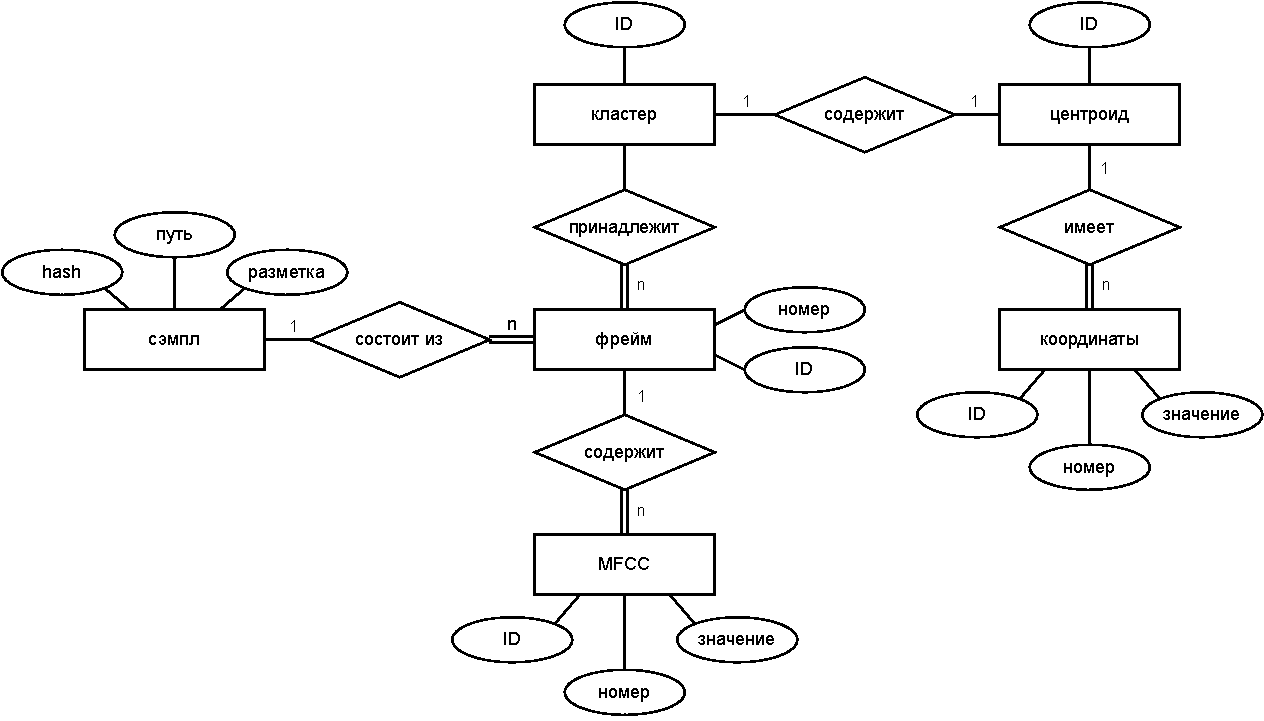
\includegraphics[width=\linewidth]{assets/chen}
	\caption{Диаграмма сущностей базы данных в нотации Чена}
	\label{fig:chen}
\end{figure} 
Сущность <<сэмпл>> представляет собой информацию о WAV-файле, который хранится в файловой системе. Сущность содержит поля, необходимые для ее обработки: уникальный хэш для идентификации сущности, абсолютный путь в файловой системе компьютера и разметка, указанная в корпусе. Звуковые дорожки разделены на небольшие фрагменты для дальнейшего анализа. Эти фрагменты представлены сущностью <<фрейм>>. Для работы с фреймами необходимо хранить информацию о его порядковом номере в сэмпле и идентификатор. 

Полученный набор фреймов используется в качестве входных данных для кластеризации. В результате кластеризации каждому фрейму присвоен кластер. Сущность базы данных, хранящая кластер, содержит уникальный идентификатор и информацию о своем центроиде. Центроид, в свою очередь, также содержит идентификатор и набор координат.
\section{Физические компоненты системы и их размещение на устройствах}
Здесь диаграмма развертывания
%Программное обеспечение следует разделить на три логических компонента: выделение информативных признаков сигнала, кластеризация и обучение скрытых марковских моделей. Из набора данных DUSHA следует выделить равное количество аудиозаписей для каждого маркера разметки. Аудиозаписи, используемые в процессе обучения, предлагается взять примерно равной длины (1.5 секунд $\pm$ 20 миллисекунд). Аудиозаписи перед обучением должны быть разделены на кадры длины 20 миллисекунд с перекрытием 50\% и кластеризованы.